\documentclass[twoside]{book}

% Packages required by doxygen
\usepackage{calc}
\usepackage{doxygen}
\usepackage{graphicx}
\usepackage[utf8]{inputenc}
\usepackage{makeidx}
\usepackage{multicol}
\usepackage{multirow}
\usepackage{textcomp}
\usepackage[table]{xcolor}

% Font selection
\usepackage[T1]{fontenc}
\usepackage{mathptmx}
\usepackage[scaled=.90]{helvet}
\usepackage{courier}
\usepackage{amssymb}
\usepackage{sectsty}
\renewcommand{\familydefault}{\sfdefault}
\allsectionsfont{%
  \fontseries{bc}\selectfont%
  \color{darkgray}%
}
\renewcommand{\DoxyLabelFont}{%
  \fontseries{bc}\selectfont%
  \color{darkgray}%
}

% Page & text layout
\usepackage{geometry}
\geometry{%
  a4paper,%
  top=2.5cm,%
  bottom=2.5cm,%
  left=2.5cm,%
  right=2.5cm%
}
\tolerance=750
\hfuzz=15pt
\hbadness=750
\setlength{\emergencystretch}{15pt}
\setlength{\parindent}{0cm}
\setlength{\parskip}{0.2cm}
\makeatletter
\renewcommand{\paragraph}{%
  \@startsection{paragraph}{4}{0ex}{-1.0ex}{1.0ex}{%
    \normalfont\normalsize\bfseries\SS@parafont%
  }%
}
\renewcommand{\subparagraph}{%
  \@startsection{subparagraph}{5}{0ex}{-1.0ex}{1.0ex}{%
    \normalfont\normalsize\bfseries\SS@subparafont%
  }%
}
\makeatother

% Headers & footers
\usepackage{fancyhdr}
\pagestyle{fancyplain}
\fancyhead[LE]{\fancyplain{}{\bfseries\thepage}}
\fancyhead[CE]{\fancyplain{}{}}
\fancyhead[RE]{\fancyplain{}{\bfseries\leftmark}}
\fancyhead[LO]{\fancyplain{}{\bfseries\rightmark}}
\fancyhead[CO]{\fancyplain{}{}}
\fancyhead[RO]{\fancyplain{}{\bfseries\thepage}}
\fancyfoot[LE]{\fancyplain{}{}}
\fancyfoot[CE]{\fancyplain{}{}}
\fancyfoot[RE]{\fancyplain{}{\bfseries\scriptsize Generated on Sun Sep 11 2016 11\-:10\-:44 for Byggern by Doxygen }}
\fancyfoot[LO]{\fancyplain{}{\bfseries\scriptsize Generated on Sun Sep 11 2016 11\-:10\-:44 for Byggern by Doxygen }}
\fancyfoot[CO]{\fancyplain{}{}}
\fancyfoot[RO]{\fancyplain{}{}}
\renewcommand{\footrulewidth}{0.4pt}
\renewcommand{\chaptermark}[1]{%
  \markboth{#1}{}%
}
\renewcommand{\sectionmark}[1]{%
  \markright{\thesection\ #1}%
}

% Indices & bibliography
\usepackage{natbib}
\usepackage[titles]{tocloft}
\setcounter{tocdepth}{3}
\setcounter{secnumdepth}{5}
\makeindex

% Hyperlinks (required, but should be loaded last)
\usepackage{ifpdf}
\ifpdf
  \usepackage[pdftex,pagebackref=true]{hyperref}
\else
  \usepackage[ps2pdf,pagebackref=true]{hyperref}
\fi
\hypersetup{%
  colorlinks=true,%
  linkcolor=blue,%
  citecolor=blue,%
  unicode%
}

% Custom commands
\newcommand{\clearemptydoublepage}{%
  \newpage{\pagestyle{empty}\cleardoublepage}%
}


%===== C O N T E N T S =====

\begin{document}

% Titlepage & ToC
\hypersetup{pageanchor=false}
\pagenumbering{roman}
\begin{titlepage}
\vspace*{7cm}
\begin{center}%
{\Large Byggern }\\
\vspace*{1cm}
{\large Generated by Doxygen 1.8.6}\\
\vspace*{0.5cm}
{\small Sun Sep 11 2016 11:10:44}\\
\end{center}
\end{titlepage}
\clearemptydoublepage
\tableofcontents
\clearemptydoublepage
\pagenumbering{arabic}
\hypersetup{pageanchor=true}

%--- Begin generated contents ---
\chapter{Byggern}
\label{md__r_e_a_d_m_e}
\hypertarget{md__r_e_a_d_m_e}{}
This is the Byggern project...

This team is made up of Johan Lofstad, Sondre Baugstø and Sondre Vincent Russvoll. 



Documentation is available at \href{https://srussvoll.github.io/byggern/}{\tt https\-://srussvoll.\-github.\-io/byggern/}. 



The 'build' folder contains all build files like .hex and .elf. The 'include' folder contains all header files. The 'lib' folder contains folders with libraries containing both source and header files. The 'src' folder contains the source files. 



Added C++ support. Note that the S\-T\-L isn't implemented. More specifically, only the C standard library is available... The new and delete operators are not implemented either, so just don't use dynamic allocation without malloc(). Also remember that I\-S\-Rs are implemented in C with no support for overloading... Because of this interrupt handlers must be friends of the originator class. 
\chapter{Hierarchical Index}
\section{Class Hierarchy}
This inheritance list is sorted roughly, but not completely, alphabetically\+:\begin{DoxyCompactList}
\item \contentsline{section}{Menu\+:\+:Controller}{\pageref{class_menu_1_1_controller}}{}
\item \contentsline{section}{Menu\+:\+:Item}{\pageref{struct_menu_1_1_item}}{}
\item \contentsline{section}{Menu\+:\+:Menu}{\pageref{struct_menu_1_1_menu}}{}
\item \contentsline{section}{Stream}{\pageref{class_stream}}{}
\begin{DoxyCompactList}
\item \contentsline{section}{A\+DC}{\pageref{class_a_d_c}}{}
\item \contentsline{section}{O\+L\+ED}{\pageref{class_o_l_e_d}}{}
\item \contentsline{section}{U\+A\+RT}{\pageref{class_u_a_r_t}}{}
\end{DoxyCompactList}
\end{DoxyCompactList}

\chapter{Class Index}
\section{Class List}
Here are the classes, structs, unions and interfaces with brief descriptions\-:\begin{DoxyCompactList}
\item\contentsline{section}{\hyperlink{class_stream}{Stream} }{\pageref{class_stream}}{}
\item\contentsline{section}{\hyperlink{class_test_stream}{Test\-Stream} }{\pageref{class_test_stream}}{}
\end{DoxyCompactList}

\chapter{File Index}
\section{File List}
Here is a list of all documented files with brief descriptions\-:\begin{DoxyCompactList}
\item\contentsline{section}{include/{\bfseries init.\-h} }{\pageref{init_8h}}{}
\item\contentsline{section}{lib/adc/{\bfseries adc.\-h} }{\pageref{adc_8h}}{}
\item\contentsline{section}{lib/can/{\bfseries can.\-h} }{\pageref{can_8h}}{}
\item\contentsline{section}{lib/mcp2515/{\bfseries mcp2515.\-h} }{\pageref{mcp2515_8h}}{}
\item\contentsline{section}{lib/mcp2515/{\bfseries mcp2515\-\_\-regisers.\-h} }{\pageref{mcp2515__regisers_8h}}{}
\item\contentsline{section}{lib/menu/{\bfseries menu.\-h} }{\pageref{menu_8h}}{}
\item\contentsline{section}{lib/oled/\hyperlink{oled_8h}{oled.\-h} }{\pageref{oled_8h}}{}
\item\contentsline{section}{lib/spi/\hyperlink{spi_8h}{spi.\-h} }{\pageref{spi_8h}}{}
\item\contentsline{section}{lib/stream/\hyperlink{stream_8h}{stream.\-h} }{\pageref{stream_8h}}{}
\item\contentsline{section}{lib/uart/\hyperlink{uart_8h}{uart.\-h} }{\pageref{uart_8h}}{}
\item\contentsline{section}{lib/utilities/{\bfseries fonts.\-h} }{\pageref{fonts_8h}}{}
\item\contentsline{section}{lib/utilities/{\bfseries memory.\-h} }{\pageref{memory_8h}}{}
\item\contentsline{section}{lib/utilities/{\bfseries new.\-h} }{\pageref{new_8h}}{}
\item\contentsline{section}{lib/utilities/{\bfseries printf.\-h} }{\pageref{printf_8h}}{}
\item\contentsline{section}{lib/utilities/{\bfseries utilities.\-h} }{\pageref{utilities_8h}}{}
\end{DoxyCompactList}

\chapter{Class Documentation}
\hypertarget{class_stream}{\section{Stream Class Reference}
\label{class_stream}\index{Stream@{Stream}}
}
Inheritance diagram for Stream\-:\begin{figure}[H]
\begin{center}
\leavevmode
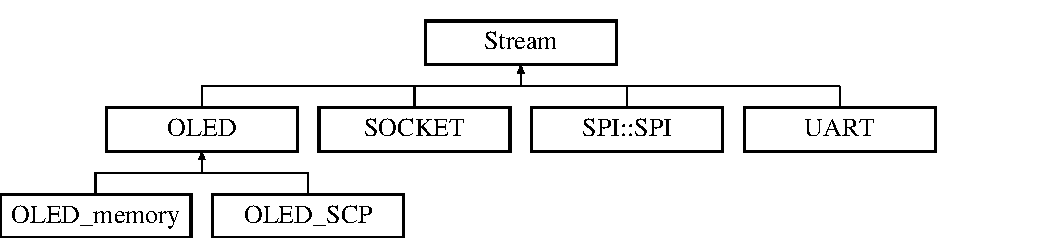
\includegraphics[height=2.000000cm]{class_stream}
\end{center}
\end{figure}
\subsection*{Public Member Functions}
\begin{DoxyCompactItemize}
\item 
\hyperlink{class_stream_afd83bbd749c467ad3dd85e1b80170c9b}{Stream} (uint8\-\_\-t $\ast$\hyperlink{class_stream_aaa6b266a85844345faee432d0267c6ec}{input\-\_\-stream}, uint16\-\_\-t \hyperlink{class_stream_a8a754b0acc9552d1b78de92b2476f4cb}{input\-\_\-stream\-\_\-size}, uint8\-\_\-t $\ast$\hyperlink{class_stream_ab2d136f405b24e5eb2a6058b24fabfa3}{output\-\_\-stream}, uint16\-\_\-t \hyperlink{class_stream_a3a171d646ab70eeb9c034aecb3a72003}{output\-\_\-stream\-\_\-size})
\item 
virtual void \hyperlink{class_stream_a508be3423e4d99ab2757275fb723002a}{Write} (uint8\-\_\-t $\ast$string, uint16\-\_\-t size)
\item 
virtual void \hyperlink{class_stream_a4f3ec0f7a24ddcfd054566feb614afba}{Read} (uint8\-\_\-t $\ast$string, uint16\-\_\-t size)
\item 
virtual uint8\-\_\-t \hyperlink{class_stream_aeb3f1b3d55f4b502c02d73ce4de42714}{Read\-Byte} ()
\item 
virtual void \hyperlink{class_stream_aeaed767b3a8d946c6f81465fa83ff17f}{Write\-Byte} (uint8\-\_\-t byte)
\item 
virtual uint8\-\_\-t \hyperlink{class_stream_a6a16ddb03d3360cef4daf4d38245091d}{Get\-Available\-Write\-Bytes} ()
\item 
virtual uint8\-\_\-t \hyperlink{class_stream_a71cec6c46f3d50cc3ab420e93ae434e1}{Get\-Available\-Read\-Bytes} ()
\item 
virtual bool \hyperlink{class_stream_a088c4e68d568acfad715c56f408fe9f8}{Check\-Input\-Overflow\-Flag} ()
\item 
virtual bool \hyperlink{class_stream_aee6c201819b874c5934a270592d9d311}{Check\-Output\-Overflow\-Flag} ()
\end{DoxyCompactItemize}
\subsection*{Protected Member Functions}
\begin{DoxyCompactItemize}
\item 
virtual void \hyperlink{class_stream_add5927208d603b08341f8972652d9c44}{Read\-From\-Buffer} (uint8\-\_\-t $\ast$buffer, uint16\-\_\-t \&start\-\_\-index, uint16\-\_\-t \&stop\-\_\-index, uint16\-\_\-t \&buffer\-\_\-size, uint8\-\_\-t $\ast$string, uint16\-\_\-t \&string\-\_\-size)
\item 
virtual void \hyperlink{class_stream_a456d59b1944143a8e4a977b8861d42ea}{Write\-To\-Buffer} (uint8\-\_\-t $\ast$buffer, uint16\-\_\-t \&start\-\_\-index, uint16\-\_\-t \&stop\-\_\-index, uint16\-\_\-t \&buffer\-\_\-size, bool \&overflow\-\_\-flag, uint8\-\_\-t $\ast$string, uint16\-\_\-t \&string\-\_\-size)
\item 
virtual uint8\-\_\-t \hyperlink{class_stream_a6c49bb8565d238e13c3ca3e9eddcf38e}{Read\-Byte\-From\-Buffer} (uint8\-\_\-t $\ast$buffer, uint16\-\_\-t \&start\-\_\-index, uint16\-\_\-t \&stop\-\_\-index, uint16\-\_\-t \&buffer\-\_\-size)
\item 
virtual void \hyperlink{class_stream_a129f3c3e763ceab692bdde38fdc89402}{Write\-Byte\-To\-Buffer} (uint8\-\_\-t $\ast$buffer, uint16\-\_\-t \&start\-\_\-index, uint16\-\_\-t \&stop\-\_\-index, uint16\-\_\-t \&buffer\-\_\-size, bool \&overflow\-\_\-flag, uint8\-\_\-t \&byte)
\item 
virtual void \hyperlink{class_stream_a70108ab0e811c6cab2636bf7afeb5e14}{Write\-Byte\-To\-Input\-Stream} (uint8\-\_\-t byte)
\item 
virtual uint8\-\_\-t \hyperlink{class_stream_a712a8e0c6659799b1bb2999b53bd983d}{Read\-Byte\-From\-Output\-Stream} ()
\item 
virtual void \hyperlink{class_stream_aa2f020721d273ce821ccf626e5eb773c}{Write\-To\-Input\-Stream} (uint8\-\_\-t $\ast$string, uint16\-\_\-t size)
\item 
virtual void \hyperlink{class_stream_adce437b86a098710237ac7dcccd5508d}{Read\-From\-Output\-Stream} (uint8\-\_\-t $\ast$string, uint16\-\_\-t size)
\item 
virtual uint16\-\_\-t \hyperlink{class_stream_a8abdeaae6339d9873842a951843cb386}{Calculate\-Length} (uint16\-\_\-t \&start\-\_\-index, uint16\-\_\-t \&stop\-\_\-index, uint16\-\_\-t \&buffer\-\_\-size)
\item 
virtual uint16\-\_\-t \hyperlink{class_stream_ac9d4705ce8fe5c9ac473939fcac423f6}{Get\-Input\-Stream\-Length} ()
\item 
virtual uint16\-\_\-t \hyperlink{class_stream_a6378bb812d0b77890926d1c724140146}{Get\-Output\-Stream\-Length} ()
\end{DoxyCompactItemize}
\subsection*{Protected Attributes}
\begin{DoxyCompactItemize}
\item 
uint8\-\_\-t $\ast$ \hyperlink{class_stream_aaa6b266a85844345faee432d0267c6ec}{input\-\_\-stream} = nullptr
\item 
uint8\-\_\-t $\ast$ \hyperlink{class_stream_ab2d136f405b24e5eb2a6058b24fabfa3}{output\-\_\-stream} = nullptr
\item 
uint16\-\_\-t \hyperlink{class_stream_ade2d5afb993214626e7c7d66cb76cd46}{input\-\_\-stream\-\_\-start\-\_\-index} = 0
\item 
uint16\-\_\-t \hyperlink{class_stream_a7406f5db92c18f0a6d7dcc924a6122cc}{output\-\_\-stream\-\_\-start\-\_\-index} = 0
\item 
uint16\-\_\-t \hyperlink{class_stream_a52cf2f675dd7ec342615e82cc29513de}{input\-\_\-stream\-\_\-stop\-\_\-index} = 0
\item 
uint16\-\_\-t \hyperlink{class_stream_ac3b2282b5977151124aa77c2d4e411ec}{output\-\_\-stream\-\_\-stop\-\_\-index} = 0
\item 
uint16\-\_\-t \hyperlink{class_stream_a3a171d646ab70eeb9c034aecb3a72003}{output\-\_\-stream\-\_\-size} = 0
\item 
uint16\-\_\-t \hyperlink{class_stream_a8a754b0acc9552d1b78de92b2476f4cb}{input\-\_\-stream\-\_\-size} = 0
\item 
bool \hyperlink{class_stream_aeffd88d8ca71bf0d084ded2a251e3a57}{input\-\_\-stream\-\_\-overflowed} = false
\item 
bool \hyperlink{class_stream_a91eb40b21c46bd57b61811a890ac047a}{output\-\_\-stream\-\_\-overflowed} = false
\end{DoxyCompactItemize}


\subsection{Constructor \& Destructor Documentation}
\hypertarget{class_stream_afd83bbd749c467ad3dd85e1b80170c9b}{\index{Stream@{Stream}!Stream@{Stream}}
\index{Stream@{Stream}!Stream@{Stream}}
\subsubsection[{Stream}]{\setlength{\rightskip}{0pt plus 5cm}Stream\-::\-Stream (
\begin{DoxyParamCaption}
\item[{uint8\-\_\-t $\ast$}]{input\-\_\-stream, }
\item[{uint16\-\_\-t}]{input\-\_\-stream\-\_\-size, }
\item[{uint8\-\_\-t $\ast$}]{output\-\_\-stream, }
\item[{uint16\-\_\-t}]{output\-\_\-stream\-\_\-size}
\end{DoxyParamCaption}
)\hspace{0.3cm}{\ttfamily [inline]}}}\label{class_stream_afd83bbd749c467ad3dd85e1b80170c9b}
The constructor. Needed to initialize stream sizes 
\begin{DoxyParams}{Parameters}
{\em input\-\_\-stream\-\_\-size} & The size of the input ring buffer. \\
\hline
{\em output\-\_\-stream\-\_\-size} & The size of the output ring buffer. \\
\hline
\end{DoxyParams}


\subsection{Member Function Documentation}
\hypertarget{class_stream_a8abdeaae6339d9873842a951843cb386}{\index{Stream@{Stream}!Calculate\-Length@{Calculate\-Length}}
\index{Calculate\-Length@{Calculate\-Length}!Stream@{Stream}}
\subsubsection[{Calculate\-Length}]{\setlength{\rightskip}{0pt plus 5cm}uint16\-\_\-t Stream\-::\-Calculate\-Length (
\begin{DoxyParamCaption}
\item[{uint16\-\_\-t \&}]{start\-\_\-index, }
\item[{uint16\-\_\-t \&}]{stop\-\_\-index, }
\item[{uint16\-\_\-t \&}]{buffer\-\_\-size}
\end{DoxyParamCaption}
)\hspace{0.3cm}{\ttfamily [protected]}, {\ttfamily [virtual]}}}\label{class_stream_a8abdeaae6339d9873842a951843cb386}
Calculates the length of the readable part of the buffer 
\begin{DoxyParams}{Parameters}
{\em start\-\_\-index} & The start index of the buffer \\
\hline
{\em stop\-\_\-index} & The stop index of the buffer \\
\hline
\end{DoxyParams}
\begin{DoxyReturn}{Returns}
Length of valid data 
\end{DoxyReturn}
\hypertarget{class_stream_a088c4e68d568acfad715c56f408fe9f8}{\index{Stream@{Stream}!Check\-Input\-Overflow\-Flag@{Check\-Input\-Overflow\-Flag}}
\index{Check\-Input\-Overflow\-Flag@{Check\-Input\-Overflow\-Flag}!Stream@{Stream}}
\subsubsection[{Check\-Input\-Overflow\-Flag}]{\setlength{\rightskip}{0pt plus 5cm}bool Stream\-::\-Check\-Input\-Overflow\-Flag (
\begin{DoxyParamCaption}
{}
\end{DoxyParamCaption}
)\hspace{0.3cm}{\ttfamily [virtual]}}}\label{class_stream_a088c4e68d568acfad715c56f408fe9f8}
Checks whether or not the input overflow flag has been set. If it has, it conducts the nessesary procedures to clear out the overflow \hypertarget{class_stream_aee6c201819b874c5934a270592d9d311}{\index{Stream@{Stream}!Check\-Output\-Overflow\-Flag@{Check\-Output\-Overflow\-Flag}}
\index{Check\-Output\-Overflow\-Flag@{Check\-Output\-Overflow\-Flag}!Stream@{Stream}}
\subsubsection[{Check\-Output\-Overflow\-Flag}]{\setlength{\rightskip}{0pt plus 5cm}bool Stream\-::\-Check\-Output\-Overflow\-Flag (
\begin{DoxyParamCaption}
{}
\end{DoxyParamCaption}
)\hspace{0.3cm}{\ttfamily [virtual]}}}\label{class_stream_aee6c201819b874c5934a270592d9d311}
Checks whether or not the output overflow flag has been set. If it has, it conducts the nessesary procedures to clear out the overflow \hypertarget{class_stream_a71cec6c46f3d50cc3ab420e93ae434e1}{\index{Stream@{Stream}!Get\-Available\-Read\-Bytes@{Get\-Available\-Read\-Bytes}}
\index{Get\-Available\-Read\-Bytes@{Get\-Available\-Read\-Bytes}!Stream@{Stream}}
\subsubsection[{Get\-Available\-Read\-Bytes}]{\setlength{\rightskip}{0pt plus 5cm}uint8\-\_\-t Stream\-::\-Get\-Available\-Read\-Bytes (
\begin{DoxyParamCaption}
{}
\end{DoxyParamCaption}
)\hspace{0.3cm}{\ttfamily [virtual]}}}\label{class_stream_a71cec6c46f3d50cc3ab420e93ae434e1}
Simply returns the number of bytes available for reading (the actual data available for receiving in the buffer) \hypertarget{class_stream_a6a16ddb03d3360cef4daf4d38245091d}{\index{Stream@{Stream}!Get\-Available\-Write\-Bytes@{Get\-Available\-Write\-Bytes}}
\index{Get\-Available\-Write\-Bytes@{Get\-Available\-Write\-Bytes}!Stream@{Stream}}
\subsubsection[{Get\-Available\-Write\-Bytes}]{\setlength{\rightskip}{0pt plus 5cm}uint8\-\_\-t Stream\-::\-Get\-Available\-Write\-Bytes (
\begin{DoxyParamCaption}
{}
\end{DoxyParamCaption}
)\hspace{0.3cm}{\ttfamily [virtual]}}}\label{class_stream_a6a16ddb03d3360cef4daf4d38245091d}
Simply returns the number of bytes available in the output buffer. The output depends on the maximum bytes allocated in the implementation. \hypertarget{class_stream_ac9d4705ce8fe5c9ac473939fcac423f6}{\index{Stream@{Stream}!Get\-Input\-Stream\-Length@{Get\-Input\-Stream\-Length}}
\index{Get\-Input\-Stream\-Length@{Get\-Input\-Stream\-Length}!Stream@{Stream}}
\subsubsection[{Get\-Input\-Stream\-Length}]{\setlength{\rightskip}{0pt plus 5cm}uint16\-\_\-t Stream\-::\-Get\-Input\-Stream\-Length (
\begin{DoxyParamCaption}
{}
\end{DoxyParamCaption}
)\hspace{0.3cm}{\ttfamily [protected]}, {\ttfamily [virtual]}}}\label{class_stream_ac9d4705ce8fe5c9ac473939fcac423f6}
Calculates the length of the readable part of the buffer 
\begin{DoxyParams}{Parameters}
{\em start\-\_\-index} & The start index of the buffer \\
\hline
{\em stop\-\_\-index} & The stop index of the buffer \\
\hline
\end{DoxyParams}
\begin{DoxyReturn}{Returns}
Length of valid data 
\end{DoxyReturn}
\hypertarget{class_stream_a6378bb812d0b77890926d1c724140146}{\index{Stream@{Stream}!Get\-Output\-Stream\-Length@{Get\-Output\-Stream\-Length}}
\index{Get\-Output\-Stream\-Length@{Get\-Output\-Stream\-Length}!Stream@{Stream}}
\subsubsection[{Get\-Output\-Stream\-Length}]{\setlength{\rightskip}{0pt plus 5cm}uint16\-\_\-t Stream\-::\-Get\-Output\-Stream\-Length (
\begin{DoxyParamCaption}
{}
\end{DoxyParamCaption}
)\hspace{0.3cm}{\ttfamily [protected]}, {\ttfamily [virtual]}}}\label{class_stream_a6378bb812d0b77890926d1c724140146}
Calculates the length of the readable part of the buffer \begin{DoxyReturn}{Returns}
Length of valid data 
\end{DoxyReturn}
\hypertarget{class_stream_a4f3ec0f7a24ddcfd054566feb614afba}{\index{Stream@{Stream}!Read@{Read}}
\index{Read@{Read}!Stream@{Stream}}
\subsubsection[{Read}]{\setlength{\rightskip}{0pt plus 5cm}void Stream\-::\-Read (
\begin{DoxyParamCaption}
\item[{uint8\-\_\-t $\ast$}]{string, }
\item[{uint16\-\_\-t}]{size}
\end{DoxyParamCaption}
)\hspace{0.3cm}{\ttfamily [virtual]}}}\label{class_stream_a4f3ec0f7a24ddcfd054566feb614afba}
Reads data from the input stream and stores in the specified data. 
\begin{DoxyParams}{Parameters}
{\em string} & Where the data should be stored \\
\hline
{\em size} & Size of the data \\
\hline
\end{DoxyParams}
\hypertarget{class_stream_aeb3f1b3d55f4b502c02d73ce4de42714}{\index{Stream@{Stream}!Read\-Byte@{Read\-Byte}}
\index{Read\-Byte@{Read\-Byte}!Stream@{Stream}}
\subsubsection[{Read\-Byte}]{\setlength{\rightskip}{0pt plus 5cm}uint8\-\_\-t Stream\-::\-Read\-Byte (
\begin{DoxyParamCaption}
{}
\end{DoxyParamCaption}
)\hspace{0.3cm}{\ttfamily [virtual]}}}\label{class_stream_aeb3f1b3d55f4b502c02d73ce4de42714}
Reads one byte from the input stream \hypertarget{class_stream_a6c49bb8565d238e13c3ca3e9eddcf38e}{\index{Stream@{Stream}!Read\-Byte\-From\-Buffer@{Read\-Byte\-From\-Buffer}}
\index{Read\-Byte\-From\-Buffer@{Read\-Byte\-From\-Buffer}!Stream@{Stream}}
\subsubsection[{Read\-Byte\-From\-Buffer}]{\setlength{\rightskip}{0pt plus 5cm}uint8\-\_\-t Stream\-::\-Read\-Byte\-From\-Buffer (
\begin{DoxyParamCaption}
\item[{uint8\-\_\-t $\ast$}]{buffer, }
\item[{uint16\-\_\-t \&}]{start\-\_\-index, }
\item[{uint16\-\_\-t \&}]{stop\-\_\-index, }
\item[{uint16\-\_\-t \&}]{buffer\-\_\-size}
\end{DoxyParamCaption}
)\hspace{0.3cm}{\ttfamily [protected]}, {\ttfamily [virtual]}}}\label{class_stream_a6c49bb8565d238e13c3ca3e9eddcf38e}
Reads a byte from the given buffer 
\begin{DoxyParams}{Parameters}
{\em buffer} & The buffer to read from \\
\hline
{\em start\-\_\-index} & The first valid bit of the buffer \\
\hline
{\em stop\-\_\-index} & The last valid bit of the buffer \\
\hline
{\em size} & The size of the buffer \\
\hline
\end{DoxyParams}
\begin{DoxyReturn}{Returns}
The byte that was read 
\end{DoxyReturn}
\hypertarget{class_stream_a712a8e0c6659799b1bb2999b53bd983d}{\index{Stream@{Stream}!Read\-Byte\-From\-Output\-Stream@{Read\-Byte\-From\-Output\-Stream}}
\index{Read\-Byte\-From\-Output\-Stream@{Read\-Byte\-From\-Output\-Stream}!Stream@{Stream}}
\subsubsection[{Read\-Byte\-From\-Output\-Stream}]{\setlength{\rightskip}{0pt plus 5cm}uint8\-\_\-t Stream\-::\-Read\-Byte\-From\-Output\-Stream (
\begin{DoxyParamCaption}
{}
\end{DoxyParamCaption}
)\hspace{0.3cm}{\ttfamily [protected]}, {\ttfamily [virtual]}}}\label{class_stream_a712a8e0c6659799b1bb2999b53bd983d}
Reads a byte from the output stream \hypertarget{class_stream_add5927208d603b08341f8972652d9c44}{\index{Stream@{Stream}!Read\-From\-Buffer@{Read\-From\-Buffer}}
\index{Read\-From\-Buffer@{Read\-From\-Buffer}!Stream@{Stream}}
\subsubsection[{Read\-From\-Buffer}]{\setlength{\rightskip}{0pt plus 5cm}void Stream\-::\-Read\-From\-Buffer (
\begin{DoxyParamCaption}
\item[{uint8\-\_\-t $\ast$}]{buffer, }
\item[{uint16\-\_\-t \&}]{start\-\_\-index, }
\item[{uint16\-\_\-t \&}]{stop\-\_\-index, }
\item[{uint16\-\_\-t \&}]{buffer\-\_\-size, }
\item[{uint8\-\_\-t $\ast$}]{string, }
\item[{uint16\-\_\-t \&}]{string\-\_\-size}
\end{DoxyParamCaption}
)\hspace{0.3cm}{\ttfamily [protected]}, {\ttfamily [virtual]}}}\label{class_stream_add5927208d603b08341f8972652d9c44}
Reads a string from the given buffer. 
\begin{DoxyParams}{Parameters}
{\em buffer} & Buffer to read from \\
\hline
{\em start\-\_\-index} & The first valid byte of the buffer \\
\hline
{\em stop\-\_\-index} & The last valid byte of the buffer \\
\hline
{\em size} & The size of the buffer \\
\hline
{\em string} & The string to read into \\
\hline
{\em length} & The length of the string \\
\hline
\end{DoxyParams}
\hypertarget{class_stream_adce437b86a098710237ac7dcccd5508d}{\index{Stream@{Stream}!Read\-From\-Output\-Stream@{Read\-From\-Output\-Stream}}
\index{Read\-From\-Output\-Stream@{Read\-From\-Output\-Stream}!Stream@{Stream}}
\subsubsection[{Read\-From\-Output\-Stream}]{\setlength{\rightskip}{0pt plus 5cm}void Stream\-::\-Read\-From\-Output\-Stream (
\begin{DoxyParamCaption}
\item[{uint8\-\_\-t $\ast$}]{string, }
\item[{uint16\-\_\-t}]{size}
\end{DoxyParamCaption}
)\hspace{0.3cm}{\ttfamily [protected]}, {\ttfamily [virtual]}}}\label{class_stream_adce437b86a098710237ac7dcccd5508d}
Reads data from the input stream and stores in the specified data. 
\begin{DoxyParams}{Parameters}
{\em string} & Where the data should be stored \\
\hline
{\em size} & Size of the data \\
\hline
\end{DoxyParams}
\hypertarget{class_stream_a508be3423e4d99ab2757275fb723002a}{\index{Stream@{Stream}!Write@{Write}}
\index{Write@{Write}!Stream@{Stream}}
\subsubsection[{Write}]{\setlength{\rightskip}{0pt plus 5cm}void Stream\-::\-Write (
\begin{DoxyParamCaption}
\item[{uint8\-\_\-t $\ast$}]{string, }
\item[{uint16\-\_\-t}]{size}
\end{DoxyParamCaption}
)\hspace{0.3cm}{\ttfamily [virtual]}}}\label{class_stream_a508be3423e4d99ab2757275fb723002a}
Writes the specified data to the output stream. 
\begin{DoxyParams}{Parameters}
{\em string} & Input data \\
\hline
{\em size} & Size of the input data \\
\hline
\end{DoxyParams}
\hypertarget{class_stream_aeaed767b3a8d946c6f81465fa83ff17f}{\index{Stream@{Stream}!Write\-Byte@{Write\-Byte}}
\index{Write\-Byte@{Write\-Byte}!Stream@{Stream}}
\subsubsection[{Write\-Byte}]{\setlength{\rightskip}{0pt plus 5cm}void Stream\-::\-Write\-Byte (
\begin{DoxyParamCaption}
\item[{uint8\-\_\-t}]{byte}
\end{DoxyParamCaption}
)\hspace{0.3cm}{\ttfamily [virtual]}}}\label{class_stream_aeaed767b3a8d946c6f81465fa83ff17f}
Writes one byte to the output stream \hypertarget{class_stream_a129f3c3e763ceab692bdde38fdc89402}{\index{Stream@{Stream}!Write\-Byte\-To\-Buffer@{Write\-Byte\-To\-Buffer}}
\index{Write\-Byte\-To\-Buffer@{Write\-Byte\-To\-Buffer}!Stream@{Stream}}
\subsubsection[{Write\-Byte\-To\-Buffer}]{\setlength{\rightskip}{0pt plus 5cm}void Stream\-::\-Write\-Byte\-To\-Buffer (
\begin{DoxyParamCaption}
\item[{uint8\-\_\-t $\ast$}]{buffer, }
\item[{uint16\-\_\-t \&}]{start\-\_\-index, }
\item[{uint16\-\_\-t \&}]{stop\-\_\-index, }
\item[{uint16\-\_\-t \&}]{buffer\-\_\-size, }
\item[{bool \&}]{overflow\-\_\-flag, }
\item[{uint8\-\_\-t \&}]{byte}
\end{DoxyParamCaption}
)\hspace{0.3cm}{\ttfamily [protected]}, {\ttfamily [virtual]}}}\label{class_stream_a129f3c3e763ceab692bdde38fdc89402}
Writes a byte to the buffer 
\begin{DoxyParams}{Parameters}
{\em buffer} & The buffer to write to \\
\hline
{\em start\-\_\-index} & The first valid bit of the buffer \\
\hline
{\em stop\-\_\-index} & The last valid bit of the buffer \\
\hline
{\em size} & The size of the buffer \\
\hline
{\em byte} & The byte to be written \\
\hline
{\em overflow\-\_\-flag} & A flag indicated an overflow \\
\hline
\end{DoxyParams}
\hypertarget{class_stream_a70108ab0e811c6cab2636bf7afeb5e14}{\index{Stream@{Stream}!Write\-Byte\-To\-Input\-Stream@{Write\-Byte\-To\-Input\-Stream}}
\index{Write\-Byte\-To\-Input\-Stream@{Write\-Byte\-To\-Input\-Stream}!Stream@{Stream}}
\subsubsection[{Write\-Byte\-To\-Input\-Stream}]{\setlength{\rightskip}{0pt plus 5cm}void Stream\-::\-Write\-Byte\-To\-Input\-Stream (
\begin{DoxyParamCaption}
\item[{uint8\-\_\-t}]{byte}
\end{DoxyParamCaption}
)\hspace{0.3cm}{\ttfamily [protected]}, {\ttfamily [virtual]}}}\label{class_stream_a70108ab0e811c6cab2636bf7afeb5e14}
Writes a byte to the input stream 
\begin{DoxyParams}{Parameters}
{\em byte} & The byte to be written \\
\hline
\end{DoxyParams}
\hypertarget{class_stream_a456d59b1944143a8e4a977b8861d42ea}{\index{Stream@{Stream}!Write\-To\-Buffer@{Write\-To\-Buffer}}
\index{Write\-To\-Buffer@{Write\-To\-Buffer}!Stream@{Stream}}
\subsubsection[{Write\-To\-Buffer}]{\setlength{\rightskip}{0pt plus 5cm}void Stream\-::\-Write\-To\-Buffer (
\begin{DoxyParamCaption}
\item[{uint8\-\_\-t $\ast$}]{buffer, }
\item[{uint16\-\_\-t \&}]{start\-\_\-index, }
\item[{uint16\-\_\-t \&}]{stop\-\_\-index, }
\item[{uint16\-\_\-t \&}]{buffer\-\_\-size, }
\item[{bool \&}]{overflow\-\_\-flag, }
\item[{uint8\-\_\-t $\ast$}]{string, }
\item[{uint16\-\_\-t \&}]{string\-\_\-size}
\end{DoxyParamCaption}
)\hspace{0.3cm}{\ttfamily [protected]}, {\ttfamily [virtual]}}}\label{class_stream_a456d59b1944143a8e4a977b8861d42ea}
Writes a string to the given buffer. 
\begin{DoxyParams}{Parameters}
{\em buffer} & Buffer to write to \\
\hline
{\em start\-\_\-index} & The first valid byte of the buffer \\
\hline
{\em stop\-\_\-index} & The last valid byte of the buffer \\
\hline
{\em size} & The size of the buffer \\
\hline
{\em string} & The string to read from \\
\hline
{\em length} & The length of the string \\
\hline
\end{DoxyParams}
\hypertarget{class_stream_aa2f020721d273ce821ccf626e5eb773c}{\index{Stream@{Stream}!Write\-To\-Input\-Stream@{Write\-To\-Input\-Stream}}
\index{Write\-To\-Input\-Stream@{Write\-To\-Input\-Stream}!Stream@{Stream}}
\subsubsection[{Write\-To\-Input\-Stream}]{\setlength{\rightskip}{0pt plus 5cm}void Stream\-::\-Write\-To\-Input\-Stream (
\begin{DoxyParamCaption}
\item[{uint8\-\_\-t $\ast$}]{string, }
\item[{uint16\-\_\-t}]{size}
\end{DoxyParamCaption}
)\hspace{0.3cm}{\ttfamily [protected]}, {\ttfamily [virtual]}}}\label{class_stream_aa2f020721d273ce821ccf626e5eb773c}
Writes the specified data to the output stream. 
\begin{DoxyParams}{Parameters}
{\em string} & Input data \\
\hline
{\em size} & Size of the input data \\
\hline
\end{DoxyParams}


\subsection{Member Data Documentation}
\hypertarget{class_stream_aaa6b266a85844345faee432d0267c6ec}{\index{Stream@{Stream}!input\-\_\-stream@{input\-\_\-stream}}
\index{input\-\_\-stream@{input\-\_\-stream}!Stream@{Stream}}
\subsubsection[{input\-\_\-stream}]{\setlength{\rightskip}{0pt plus 5cm}uint8\-\_\-t$\ast$ Stream\-::input\-\_\-stream = nullptr\hspace{0.3cm}{\ttfamily [protected]}}}\label{class_stream_aaa6b266a85844345faee432d0267c6ec}
Stores the input stream data \hypertarget{class_stream_aeffd88d8ca71bf0d084ded2a251e3a57}{\index{Stream@{Stream}!input\-\_\-stream\-\_\-overflowed@{input\-\_\-stream\-\_\-overflowed}}
\index{input\-\_\-stream\-\_\-overflowed@{input\-\_\-stream\-\_\-overflowed}!Stream@{Stream}}
\subsubsection[{input\-\_\-stream\-\_\-overflowed}]{\setlength{\rightskip}{0pt plus 5cm}bool Stream\-::input\-\_\-stream\-\_\-overflowed = false\hspace{0.3cm}{\ttfamily [protected]}}}\label{class_stream_aeffd88d8ca71bf0d084ded2a251e3a57}
Flag indicating whether the input stream has overflowed or not. \hypertarget{class_stream_a8a754b0acc9552d1b78de92b2476f4cb}{\index{Stream@{Stream}!input\-\_\-stream\-\_\-size@{input\-\_\-stream\-\_\-size}}
\index{input\-\_\-stream\-\_\-size@{input\-\_\-stream\-\_\-size}!Stream@{Stream}}
\subsubsection[{input\-\_\-stream\-\_\-size}]{\setlength{\rightskip}{0pt plus 5cm}uint16\-\_\-t Stream\-::input\-\_\-stream\-\_\-size = 0\hspace{0.3cm}{\ttfamily [protected]}}}\label{class_stream_a8a754b0acc9552d1b78de92b2476f4cb}
The size of the current input stream. This has to be set \hypertarget{class_stream_ade2d5afb993214626e7c7d66cb76cd46}{\index{Stream@{Stream}!input\-\_\-stream\-\_\-start\-\_\-index@{input\-\_\-stream\-\_\-start\-\_\-index}}
\index{input\-\_\-stream\-\_\-start\-\_\-index@{input\-\_\-stream\-\_\-start\-\_\-index}!Stream@{Stream}}
\subsubsection[{input\-\_\-stream\-\_\-start\-\_\-index}]{\setlength{\rightskip}{0pt plus 5cm}uint16\-\_\-t Stream\-::input\-\_\-stream\-\_\-start\-\_\-index = 0\hspace{0.3cm}{\ttfamily [protected]}}}\label{class_stream_ade2d5afb993214626e7c7d66cb76cd46}
An index that indicates where in the output stream the next bit is to be written \hypertarget{class_stream_a52cf2f675dd7ec342615e82cc29513de}{\index{Stream@{Stream}!input\-\_\-stream\-\_\-stop\-\_\-index@{input\-\_\-stream\-\_\-stop\-\_\-index}}
\index{input\-\_\-stream\-\_\-stop\-\_\-index@{input\-\_\-stream\-\_\-stop\-\_\-index}!Stream@{Stream}}
\subsubsection[{input\-\_\-stream\-\_\-stop\-\_\-index}]{\setlength{\rightskip}{0pt plus 5cm}uint16\-\_\-t Stream\-::input\-\_\-stream\-\_\-stop\-\_\-index = 0\hspace{0.3cm}{\ttfamily [protected]}}}\label{class_stream_a52cf2f675dd7ec342615e82cc29513de}
The index indicates where the input ring buffer stops having data \hypertarget{class_stream_ab2d136f405b24e5eb2a6058b24fabfa3}{\index{Stream@{Stream}!output\-\_\-stream@{output\-\_\-stream}}
\index{output\-\_\-stream@{output\-\_\-stream}!Stream@{Stream}}
\subsubsection[{output\-\_\-stream}]{\setlength{\rightskip}{0pt plus 5cm}uint8\-\_\-t$\ast$ Stream\-::output\-\_\-stream = nullptr\hspace{0.3cm}{\ttfamily [protected]}}}\label{class_stream_ab2d136f405b24e5eb2a6058b24fabfa3}
Stores the output stream data \hypertarget{class_stream_a91eb40b21c46bd57b61811a890ac047a}{\index{Stream@{Stream}!output\-\_\-stream\-\_\-overflowed@{output\-\_\-stream\-\_\-overflowed}}
\index{output\-\_\-stream\-\_\-overflowed@{output\-\_\-stream\-\_\-overflowed}!Stream@{Stream}}
\subsubsection[{output\-\_\-stream\-\_\-overflowed}]{\setlength{\rightskip}{0pt plus 5cm}bool Stream\-::output\-\_\-stream\-\_\-overflowed = false\hspace{0.3cm}{\ttfamily [protected]}}}\label{class_stream_a91eb40b21c46bd57b61811a890ac047a}
Flag indicating whether the output stream has overflowed or not. \hypertarget{class_stream_a3a171d646ab70eeb9c034aecb3a72003}{\index{Stream@{Stream}!output\-\_\-stream\-\_\-size@{output\-\_\-stream\-\_\-size}}
\index{output\-\_\-stream\-\_\-size@{output\-\_\-stream\-\_\-size}!Stream@{Stream}}
\subsubsection[{output\-\_\-stream\-\_\-size}]{\setlength{\rightskip}{0pt plus 5cm}uint16\-\_\-t Stream\-::output\-\_\-stream\-\_\-size = 0\hspace{0.3cm}{\ttfamily [protected]}}}\label{class_stream_a3a171d646ab70eeb9c034aecb3a72003}
The size of the current output stream. This has to be set \hypertarget{class_stream_a7406f5db92c18f0a6d7dcc924a6122cc}{\index{Stream@{Stream}!output\-\_\-stream\-\_\-start\-\_\-index@{output\-\_\-stream\-\_\-start\-\_\-index}}
\index{output\-\_\-stream\-\_\-start\-\_\-index@{output\-\_\-stream\-\_\-start\-\_\-index}!Stream@{Stream}}
\subsubsection[{output\-\_\-stream\-\_\-start\-\_\-index}]{\setlength{\rightskip}{0pt plus 5cm}uint16\-\_\-t Stream\-::output\-\_\-stream\-\_\-start\-\_\-index = 0\hspace{0.3cm}{\ttfamily [protected]}}}\label{class_stream_a7406f5db92c18f0a6d7dcc924a6122cc}
An index that indicates where in the input stream the next bit is to be written \hypertarget{class_stream_ac3b2282b5977151124aa77c2d4e411ec}{\index{Stream@{Stream}!output\-\_\-stream\-\_\-stop\-\_\-index@{output\-\_\-stream\-\_\-stop\-\_\-index}}
\index{output\-\_\-stream\-\_\-stop\-\_\-index@{output\-\_\-stream\-\_\-stop\-\_\-index}!Stream@{Stream}}
\subsubsection[{output\-\_\-stream\-\_\-stop\-\_\-index}]{\setlength{\rightskip}{0pt plus 5cm}uint16\-\_\-t Stream\-::output\-\_\-stream\-\_\-stop\-\_\-index = 0\hspace{0.3cm}{\ttfamily [protected]}}}\label{class_stream_ac3b2282b5977151124aa77c2d4e411ec}
The index indicates where the output ring buffer stops having data 

The documentation for this class was generated from the following files\-:\begin{DoxyCompactItemize}
\item 
lib/stream/\hyperlink{stream_8h}{stream.\-h}\item 
lib/stream/stream.\-cpp\end{DoxyCompactItemize}

\hypertarget{class_test_stream}{\section{Test\-Stream Class Reference}
\label{class_test_stream}\index{Test\-Stream@{Test\-Stream}}
}
Inheritance diagram for Test\-Stream\-:\begin{figure}[H]
\begin{center}
\leavevmode
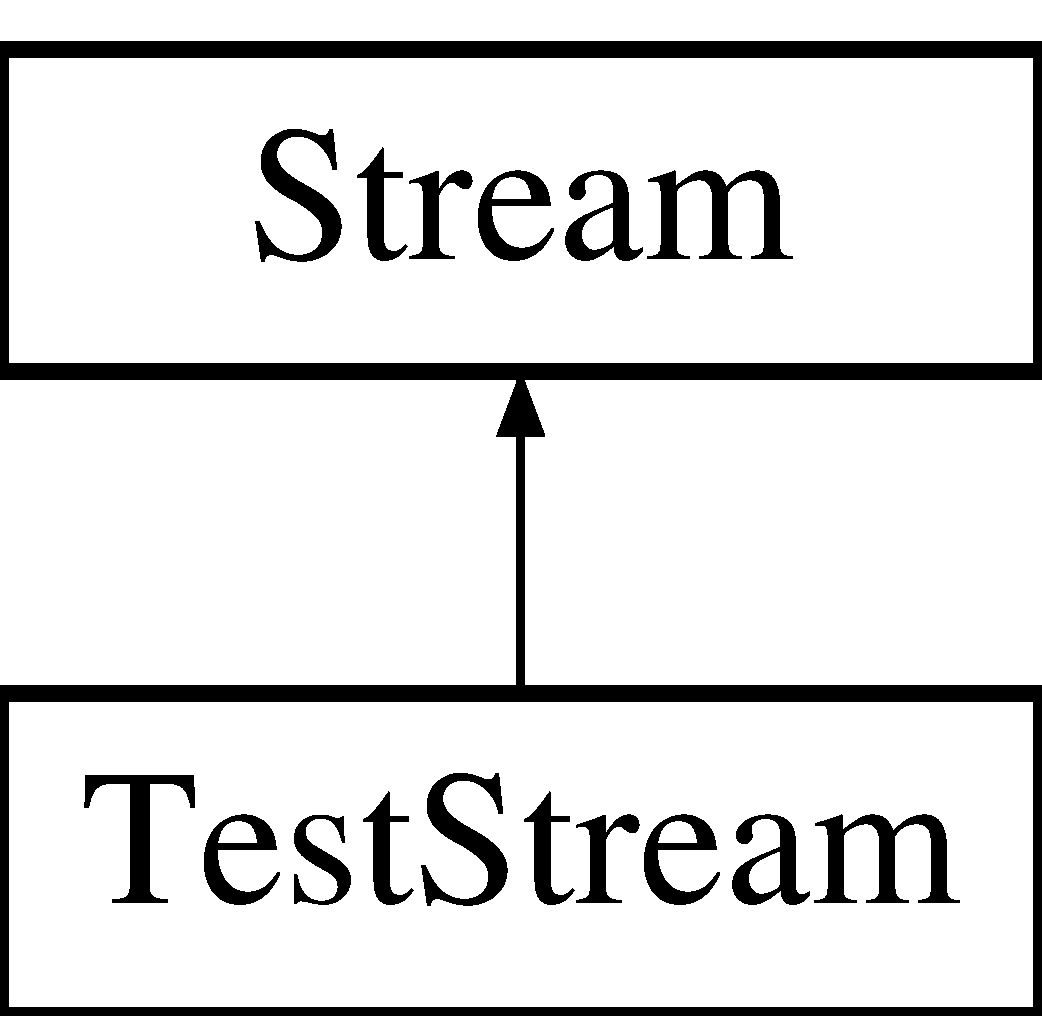
\includegraphics[height=2.000000cm]{class_test_stream}
\end{center}
\end{figure}
\subsection*{Private Attributes}
\begin{DoxyCompactItemize}
\item 
\hypertarget{class_test_stream_a4fbf64a4b85e5973859e849bf0799456}{uint8\-\_\-t {\bfseries input\-\_\-stream} \mbox{[}10\mbox{]}}\label{class_test_stream_a4fbf64a4b85e5973859e849bf0799456}

\item 
\hypertarget{class_test_stream_aa211bf4c182b5304ee2f841379e23f96}{uint8\-\_\-t {\bfseries output\-\_\-stream} \mbox{[}10\mbox{]}}\label{class_test_stream_aa211bf4c182b5304ee2f841379e23f96}

\end{DoxyCompactItemize}
\subsection*{Additional Inherited Members}


The documentation for this class was generated from the following files\-:\begin{DoxyCompactItemize}
\item 
lib/\-Test\-Stream/Test\-Stream.\-h\item 
lib/\-Test\-Stream/Test\-Stream.\-cpp\end{DoxyCompactItemize}

\chapter{File Documentation}
\hypertarget{stream_8h}{\section{lib/stream/stream.h File Reference}
\label{stream_8h}\index{lib/stream/stream.\-h@{lib/stream/stream.\-h}}
}
{\ttfamily \#include $<$string.\-h$>$}\\*
{\ttfamily \#include $<$avr/io.\-h$>$}\\*
\subsection*{Classes}
\begin{DoxyCompactItemize}
\item 
class \hyperlink{class_stream}{Stream}
\end{DoxyCompactItemize}


\subsection{Detailed Description}
\begin{DoxyAuthor}{Author}
Johan Lofstad, Sondre Baugstø, Sondre Russvoll 
\end{DoxyAuthor}
\begin{DoxyVersion}{Version}
1.\-0
\end{DoxyVersion}
An interface for handling streams with default methods. 
%--- End generated contents ---

% Index
\newpage
\phantomsection
\addcontentsline{toc}{chapter}{Index}
\printindex

\end{document}
